\documentclass[12pt]{article}
\usepackage{amsthm,amssymb,amsfonts,amsmath,amstext,systeme}
\usepackage{graphicx,float}
\usepackage{tabularx}

\marginparwidth 0pt
\oddsidemargin -1.2 truecm
\evensidemargin  0pt 
\marginparsep 0pt
\topmargin -2.2truecm
\linespread{1}
\textheight 25.8 truecm
\textwidth 18.5 truecm
\newenvironment{remark}{\noindent{\bf Remark }}{\vspace{0mm}}
\newenvironment{remarks}{\noindent{\bf Remarks }}{\vspace{0mm}}
\newenvironment{question}{\noindent{\bf Question }}{\vspace{0mm}}
\newenvironment{questions}{\noindent{\bf Questions }}{\vspace{0mm}}
\newenvironment{note}{\noindent{\bf Note }}{\vspace{0mm}}
\newenvironment{summary}{\noindent{\bf Summary }}{\vspace{0mm}}
\newenvironment{back}{\noindent{\bf Background}}{\vspace{0mm}}
\newenvironment{conclude}{\noindent{\bf Conclusion}}{\vspace{0mm}}
\newenvironment{concludes}{\noindent{\bf Conclusions}}{\vspace{0mm}}
\newenvironment{dill}{\noindent{\bf Description of Dill's model}}{\vspace{0mm}}
\newenvironment{maths}{\noindent{\bf Mathematics needed}}{\vspace{0mm}}
\newenvironment{inst}{\noindent{\bf Instructions}}{\vspace{0mm}}
\newenvironment{notes}{\noindent{\bf Notes }}{\vspace{0mm}}
\newenvironment{theorem}{\noindent{\bf Theorem }}{\vspace{0mm}}
\newenvironment{example}{\noindent{\bf Example }}{\vspace{0mm}}
\newenvironment{examples}{\noindent{\bf Examples }}{\vspace{0mm}}
\newenvironment{topics}{\noindent{\bf Topics}}{\vspace{0mm}}
\newenvironment{outcomes}{\noindent{\bf Expected Learning Outcomes}}{\vspace{0mm}}
\newenvironment{lemma}{\noindent{\bf Lemma }}{\vspace{0mm}}
\newenvironment{solution}{\noindent{\it Solution}}{\vspace{2mm}}
\newcommand{\ds}{\displaystyle}
\newcommand{\un}{\underline}
\newcommand{\bs}{\boldsymbol}

\begin{document}

\baselineskip 18 pt
\begin{center}
	{\large \bf HKDSE MATH M2 2013}\\
	\vspace{2 mm}

\end{center}
\vspace{0.05cm}

\begin{enumerate}
	\item \textbf{HKDSE Math M2 2013 Q1}\\
	Find $\displaystyle\frac{d}{dx} (\sin{2x})$ from first principles. \\(4 marks)


	\item \textbf{HKDSE Math M2 2013 Q2}\\
	Suppose the coefficient of $x$ and $x^2$ in the expansion of $(1+ax)^n$ are $-20$ and 180 respectively. Find the values of $a$ and $n$. \\(4 marks)


	\item \textbf{HKDSE Math M2 2013 Q3}\\
	Prove, by mathematical induction, that for all positive integers $n$, $$\displaystyle 1 + \frac{1}{1 \times 4} + \frac{1}{4 \times 7} + \frac{1}{7 \times 10} + \cdots + \frac{1}{(3n-2)(3n+1))} = \frac{4n+1}{3n+1}.$$ \\(5 marks)
		

	\item \textbf{HKDSE Math M2 2013 Q4}\\
	The slope at any point $(x,y)$ of a curve is given by $\displaystyle\frac{dy}{dx} = e^x - 1$. It is given that the curve passes through the point $(1,e)$. 
	\begin{enumerate}
		\item [(a)]Find the equation of the curve.
		\item [(b)]Find the equation of tangent to the curve at the point where the curve cuts the $y$-axis.
	\end{enumerate}
	(5 marks)

	\item \textbf{HKDSE Math M2 2013 Q5}\\
	Consider a continuous function $f(x) = \displaystyle\frac{3 -3x^2}{3+x^2}$. It is given that $$\begin{array}{|c|c|c|c|c|c|c|c|}
		\hline
		x & x<-1 & -1 & -1<x<0 & 0 & 0<x<1 & 1 & x>1\\
		\hline
		f'(x) & + & + & + & 0 & - & - & -\\
		\hline		
		f''(x) & + & 0 & - & - & - & 0 & +\\
		\hline
    \end{array}$$
	('$+$' and '$-$' denote 'positive value' and 'negative value' respectively.)
	\begin{enumerate}
		\item [(a)]Find all the maximum and/or minimum point(s) and point(s) of inflexion.
		\item [(b)]Find the asymptote(s) of the graph of $y = f(x)$. 
		\item [(c)]Sketch the graph of $y = f(x)$.
	\end{enumerate}
	(6 marks)

	\item \textbf{HKDSE Math M2 2013 Q6}\\
	Figure 1 shows the shaded region with boundaries $C : y = \displaystyle\frac{-x^2}{2} + 2x + 4$, $L_1 : y = 4$ and $L_2 : x = 5$. It is given that $C$ intersects $L_1$ at $(0,4)$ and $(4,4)$. 
	\begin{figure}[H]
		\centering
		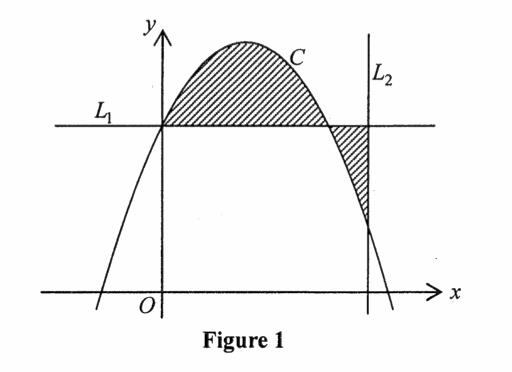
\includegraphics[width = .5\linewidth]{2013Figure1}
	\end{figure}
	\begin{enumerate}
		\item [(a)]Find the area of the shaded region.
		\item [(b)]Find the volume of solid of revolution when the shaded region is revolved about $L_1$.
	\end{enumerate}
	(6 marks)

	\item \textbf{HKDSE Math M2 2013 Q7}
	\begin{enumerate}
		\item [(a)]Prove the identity $\tan{x} = \displaystyle\frac{\sin{2x}}{1+\cos{2x}}$. 
		\item [(b)]Using (a), prove the identity $\tan{y} = \displaystyle\frac{\sin{8y}\cos{4y}\cos{2y}}{(1+\cos{8y})(1+\cos{4y})(1+\cos{2y})}$.
	\end{enumerate}
	(5 marks)

	\item \textbf{HKDSE Math M2 2013 Q8}\\
	Let $M$ be the matrix $\begin{pmatrix}
		1 & k & 0\\
		0 & 1 & 1\\
		k & 0 & 0\\
	\end{pmatrix}$, where $k \neq 0$. 
	\begin{enumerate}
		\item [(a)]Find $M^{-1}$. 
		\item [(b)]If $M\begin{pmatrix}
		x\\
		1\\
		z\\
	\end{pmatrix} = \begin{pmatrix}
		2\\
		2\\
		1\\
	\end{pmatrix}$, find the value of $k$.
	\end{enumerate}
	(5 marks)

	\item \textbf{HKDSE Math M2 2013 Q9}\\
	Consider the following system of linear equations in $x$, $y$ and $z$
		$$(E)  \left\{\begin{matrix}
		x & - & ay & + & z & = & 2\\
		2x & + & (1-2a)y & + & (2-b)z  & =  & a+4\\
		3x & + & (1-3a)y & + & (3-ab)z & = & 4\\
		\end{matrix}\right.\text{, where }a\text{ and }b\text{ are real numbers.}$$
		It is given that $(E)$ has infinitely many solutions.
	\begin{enumerate}
		\item [(a)]Find the values of $a$ and $b$.
		\item [(b)]Solve $(E)$.
	\end{enumerate}
	(5 marks)


	\item \textbf{HKDSE Math M2 2013 Q10}\\
	Let $\overrightarrow{OA} = 2\textbf{i}$ and 
	$\overrightarrow{OB} = \textbf{i} +2 \textbf{j}$. $M$ is the mid-point of $OA$ and $N$ lies on $AB$ such that $BN : NA = k: 1$. $BM$ intersects $ON$ at $P$ (see Figure 2).
	\begin{figure}[H]
		\centering
		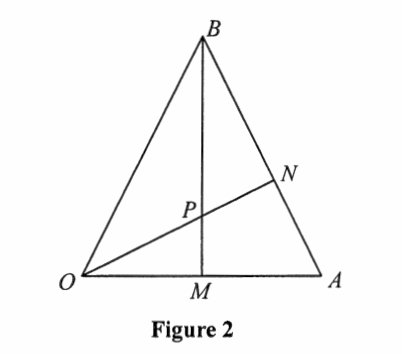
\includegraphics[width = .5\linewidth]{2013Figure2}
	\end{figure}
	\begin{enumerate}
		\item [(a)]Express $\overrightarrow{ON}$ in terms of $k$.
		\item [(b)]If $A$, $N$, $P$ and $M$ are concyclic, find the value of $k$.
	\end{enumerate}
	(5 marks)

	\item \textbf{HKDSE Math M2 2013 Q11}
	\begin{enumerate}
		\item [(a)]Let $0 < \theta < \displaystyle\frac{\pi}{2}$. By finding $\displaystyle\frac{d}{d\theta} \ln{(\sec{\theta} + \tan{\theta})}$, or otherwise, show that $\displaystyle\int\sec{\theta}\,d\theta =\ln{(\sec{\theta} + \tan{\theta})} + C$, where $C$ is any constant. \\(2 marks)
		\item [(b)]
		\begin{enumerate}
			\item [(i)]Using (a) and a suitable substitution, show that $\displaystyle\int\frac{du}{\sqrt{u^2-1}} = \ln{(u + \sqrt{u^2-1})} + C$ for $u > 1$. 
			\item [(ii)]Using (b)(i), show that $\displaystyle\int_{0}^{1}\frac{2x}{\sqrt{x^4+4x^2+3}}\,dx = \ln{(6 + 4\sqrt{2} - 3\sqrt{3} - 2\sqrt{6})}$.
		\end{enumerate}
		(5 marks)
		\item [(c)]Let $t = \tan{\phi}$. Show that $\displaystyle\frac{d\phi}{dt} = \frac{1}{1+t^2}$. \\
		Hence evaluate $\displaystyle\int_0^{\frac{\pi}{4}}\frac{\tan{\phi}}{\sqrt{1+2\cos^2{\phi}}}\,d\phi$. \\(5 marks)
	\end{enumerate}


	\item \textbf{HKDSE Math M2 2013 Q12}\\
	In Figure 3, the distance between two houses $A$ and $B$ lying on a straight river bank is 40 m. The width of the river is always 30 m. In the beginning, Mike stands at the starting point $P$ in the opposite bank which is 30 m from $A$. Mike's wife, situated at $A$, is watching him running along the bank for $x$ m at a constant speed of 7 m s$^{-1}$ to point $Q$ and then swimming at a constant speed of 1.4 m s$^{-1}$ along a straight path to reach $B$. 
	\begin{figure}[H]
		\centering
		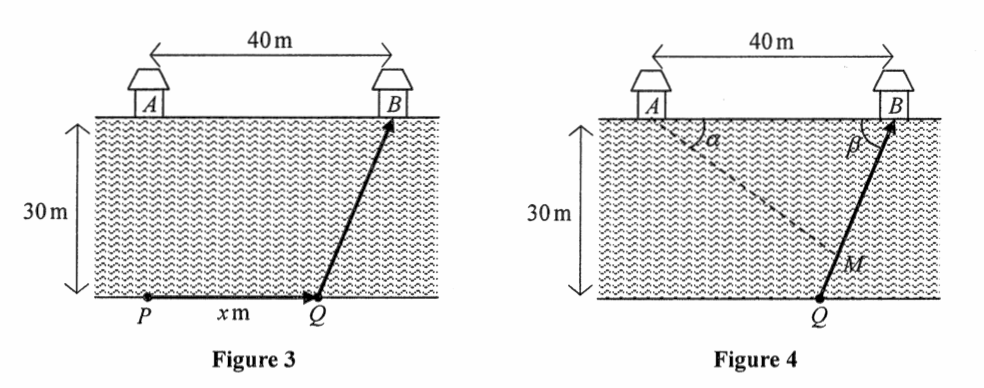
\includegraphics[width = .5\linewidth]{2013Figure3n4}
	\end{figure}
	\begin{enumerate}
		\item [(a)]Let $T$ seconds be the time that Mike travels from $P$ to $B$. 
		\begin{enumerate}
			\item [(i)]Express $T$ in terms of $x$. 
			\item [(ii)]When $T$ is minimum, show that $x$ satisfies the equation $2x^2 -160x+3125 = 0$. \\
			Hence show that $QB = \displaystyle\frac{25\sqrt{6}}{2}$ m. \\(6 marks)
		\end{enumerate}
		\item [(b)]In Figure 4, Mike is swimming from $Q$ to $B$ with $QB$ equal to the value mentioned in (a)(ii).\\
		Let $\angle MAB = \alpha$ and $\angle ABM = \beta$, where $M$ is the position of Mike.
		\begin{enumerate}
			\item [(i)]By finding $\sin{\beta}$ and $\cos{\beta}$, show that $MB = \displaystyle\frac{200\tan{\alpha}}{\tan{\alpha} + 2\sqrt{6}}$. 
			\item [(ii)]Find the rate of change of $\alpha$ when $\alpha = 0.2$ radian. Correct your answer to 4 decimal places.
		\end{enumerate}
		(7 marks)
	\end{enumerate}


	\item \textbf{HKDSE Math M2 2013 Q13}\\
	For any matrix $M = \begin{pmatrix}
		a&b\\c&d\\
	\end{pmatrix}$, define tr($M$) $= a + d$.\\
	Let $A$ and $B$ be $2 \times 2$ matrices such that $BAB^{-1} = \begin{pmatrix}
		1&0\\0&3\\
	\end{pmatrix}$. 
	\begin{enumerate}
		\item [(a)]
		\begin{enumerate}
			\item [(i)]For any matrix $N = \begin{pmatrix}
				e&f\\g&h\\
			\end{pmatrix}$, prove that $\displaystyle\text{tr}(MN) = \text{tr}(NM)$. 
			\item [(ii)]Show that $\text{tr}(A) = 4$. 
			\item [(iii)]Find the value of $|A|$.
		\end{enumerate}
		(6 marks)
		\item [(b)]Let $C = \begin{pmatrix}
			p&q\\r&s\\
		\end{pmatrix}$. It is given that $C \begin{pmatrix} x\\y\\ \end{pmatrix} = \lambda_1\begin{pmatrix} x\\y\\ \end{pmatrix}$ and $C \begin{pmatrix} x\\y\\ \end{pmatrix} = \lambda_2\begin{pmatrix} x\\y\\ \end{pmatrix}$ for some non-zero matrices $\begin{pmatrix} x\\y\\ \end{pmatrix}$ and distinct scalars $\lambda_1$ and $\lambda_2$. 
		\begin{enumerate}
			\item [(i)]Prove that $\begin{vmatrix}
				p - \lambda_1 & q \\ 
				r & s - \lambda_1   \notag
				\end{vmatrix} = 0$ and $\begin{vmatrix}
				p - \lambda_2 & q \\ 
				r & s - \lambda_2   \notag
				\end{vmatrix} = 0$. 
			\item [(ii)]Prove that $\lambda_1$ and $\lambda_2$ are the roots of the equation $\lambda^2 - \text{tr}(C) \cdot \lambda + |C| = 0$.
		\end{enumerate}
		(5 marks)
		\item [(c)]Find the two values of $\lambda$ such that $A\begin{pmatrix}
			x\\y\\
		\end{pmatrix} = \lambda \begin{pmatrix}
			x\\y\\
		\end{pmatrix}$ for some non-zero matrices $\begin{pmatrix}
			x\\y\\
		\end{pmatrix}$. \\(2 marks)
	\end{enumerate}


	\item \textbf{HKDSE Math M2 2013 Q14}\\
	Figure 5 shows a fixed tetrahedron $OABC$ with $\angle AOB = \angle BOC = \angle COA = 90^{\circ}$. $P$ is a variable point such that $\overrightarrow{AP}\cdot\overrightarrow{BP} + \overrightarrow{BP}\cdot\overrightarrow{CP} + \overrightarrow{CP}\cdot\overrightarrow{AP} = 0$. Let $D$ be the fixed point such that $\overrightarrow{OD} = \displaystyle\frac{\overrightarrow{OA}+\overrightarrow{OB}+\overrightarrow{OC}}{3}$. Let $\overrightarrow{OA} = \textbf{a}$, $\overrightarrow{OB} = \textbf{b}$, $\overrightarrow{OC} = \textbf{c}$, $\overrightarrow{OP} = \textbf{p}$ and $\overrightarrow{OD} = \textbf{d}$. 
	\begin{figure}[H]
		\centering
		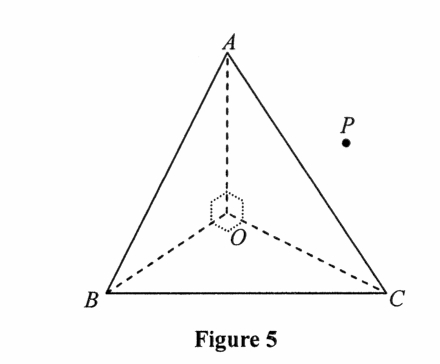
\includegraphics[width = .5\linewidth]{2013Figure5}
	\end{figure}
	\begin{enumerate}
		\item [(a)]
		\begin{enumerate}
			\item [(i)]Show that $\overrightarrow{AP}\cdot\overrightarrow{BP} = \textbf{p}\cdot\textbf{p} - (\textbf{a} + \textbf{b})\cdot\textbf{p}$. 
			\item [(ii)]Using (a)(i), show that $\textbf{p}\cdot\textbf{p} = 2\textbf{p}\cdot\textbf{d}$. 
			\item [(iii)]Show that $|\textbf{p} - \textbf{d}| = |\textbf{d}|$. \\
			Hence show that $P$ lies on the sphere centred at $D$ with fixed radius.
		\end{enumerate}
		(8 marks)
		\item [(b)]
		\begin{enumerate}
			\item [(i)]Alice claims that $O$ lies on the sphere mentioned in (a)(iii). Do you agree? Explain your answer. 
			\item [(ii)]Suppose $P_1$, $P_2$ and $P_3$ are three distinct points on the sphere in (a)(iii) such that $\overrightarrow{DP_1}\times\overrightarrow{DP_2} = \overrightarrow{DP_2}\times\overrightarrow{DP_3}$. Alice claims that the radius of the circle passing through $P_1$, $P_2$ and $P_3$ is $OD$. Do you agree? Explain your answer.
		\end{enumerate}
		(4 marks)
	\end{enumerate}
\end{enumerate}
\end{document}